\chapter{Getting started}

\section{Introduction}

This chapter gives an overview of how \dfastmi can be used.
The program can run in one of three modes:

\begin{enumerate}
\item \emph{batch mode}: in this mode the program runs the analysis without user interaction for a configuration file of which the name as command line argument,
\item \emph{cli mode}: in this (legacy) mode the configuration for the analysis is obtained by asking the user questions via a command line interface which support simulation results from WAQUA only, and
\item \emph{gui mode}: in this mode the user specifies the configuration via a graphical user interface from which the analysis can either be started directly or the configuration can be saved for batch mode execution at a later time.
\end{enumerate}

The program runs by default in the gui mode; other run modes can be selected via the command line argument.

\begin{tabular}{l|l|p{8cm}}
short & long & description \\ \hline
\keyw{-h} & \keyw{-{}-help} & show help text and exit \\
 & \keyw{-{}-rivers} & name of river configuration file (default: \keyw{Dutch\_rivers.ini}) \\
 & \keyw{-{}-language} & language selection: \keyw{NL} or \keyw{UK} (default: \keyw{UK}) \\
 & \keyw{-{}-mode} & run mode \keyw{batch}, \keyw{cli} or \keyw{gui} (default: \keyw{gui} \\
 & \keyw{-{}-config} & name of analysis configuration file \\
 & \keyw{-{}-reduced\_output} & write reduced SIMONA BOX files (applies to legacy cli mode only) \\
\end{tabular}

By default the program runs for the Dutch Rhine and Meuse river branches, but a different river configuration can be provided by means of the \keyw{-{}-rivers} command line switch; this option is supported by all run modes.
For details on the format of the river configuration file, see the appropriate section in the appendix.
The language setting influences all texts displayed by the program in cli and gui modes as well as the texts written to the report file as well as the names of the various output files.
The following list indicates the English and Dutch names:

\begin{itemize}
\item Text file with summary report of the analysis \\
English: \keyw{report.txt} \\
Dutch: \keyw{verslag.run}
\item Average yearly change in SIMONA BOX file format (when the analysis runs using WAQUA input) \\
English: \keyw{yearavg\_dzb.out} \\
Dutch: \keyw{jaargem.out}
\item Maximum change in SIMONA BOX file format (when the analysis runs using WAQUA input) \\
English: \keyw{max\_dzb.out} \\
Dutch: \keyw{maxmorf.out}
\item Minimum change in SIMONA BOX file format (when the analysis runs using WAQUA input) \\
English: \keyw{min\_dzb.out} \\
Dutch: \keyw{minmorf.out}
UGRID netCDF file containing variables for average yearly change, maximum change, and minimum change (when the analysis runs using \dflowfm input) \\
English: \keyw{dfastmi\_results.nc} \\
Dutch: \keyw{dfastmi\_resultaten.nc}
\end{itemize}

The following sections describe the three options.

\section{Running in batch mode}

The batch mode runs an analysis using either WAQUA or \dflowfm results without user interaction.
The program should be started with the run mode set to \keyw{batch} and a configuration file specified on the command line as follows

\begin{Verbatim}
> dfastmi --mode batch --config myfile.cfg
\end{Verbatim}

You may choose to run the program in either Dutch \keyw{-{}-language NL} or English \keyw{-{}-language UK}; the latter is the default.
Please note that the language does not only affect the text in the report, but also the names of the output files as indicated in the opening section of this chapter.
The content of the configuration file is described in Appendix X; it can be generated using either a text editor or \dfastmi running in gui mode.
The \keyw{-{}-reduced\_output} option for smaller SIMONA BOX file output is currently not supported in this run mode.

\section{Running in interactive command line mode}

The cli mode runs an interactive command line analysis using WAQUA results; this run mode does not support \dflowfm files.
The program should be started with the run mode set to \keyw{cli} on the command line as follows

\begin{Verbatim}
> dfastmi --mode cli
\end{Verbatim}

You may choose to run the program in either Dutch \keyw{-{}-language NL} or English \keyw{-{}-language UK}; the latter is the default.
Please note that the language does not only affect the text in the report, but also the names of the output files as indicated in the opening section of this chapter.
You may also choose to select the \keyw{-{}-reduced\_output} option for smaller SIMONA BOX file output.
Although this is an interactive run mode, you may use this mode also as a batch mode by redirecting standard input to read from file as follows

\begin{Verbatim}
> dfastmi --mode cli < myfile.in
\end{Verbatim}

In this case each line in the file \file{myfile.in} should contain the appropriate answer to the question.
This run mode is included for backward compatibility and comparison with its predecessor WAQMORF.
We recommend to use either the gui mode or the batch mode instead.

\section{Running in gui mode}

This is the default mode for the program, so no command line argument needed.
It supports analysis using either WAQUA or \dflowfm results.
As with the other run modes, you may choose to run the program in either Dutch \keyw{-{}-language NL} or English \keyw{-{}-language UK}; the latter is the default.
Please note that the language does not only affect the text in the report, but also the names of the output files as indicated in the opening section of this chapter.
Furthermore, you may specify a configuration file to load upon start.
For example

\begin{Verbatim}
> dfastmi --language NL --config myfile.cfg
\end{Verbatim}

runs the program in Dutch and loads the myfile.cfg configuration file into the graphical user interface.
The \keyw{-{}-reduced\_output} option for smaller SIMONA BOX file output is currently not supported in this run mode.

\begin{figure}
\center
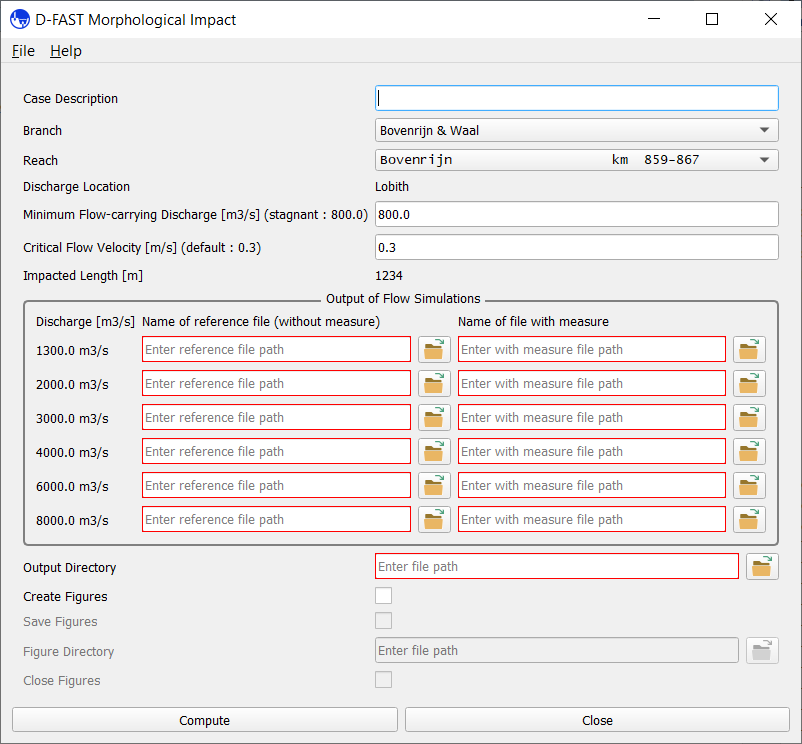
\includegraphics[width=12cm]{figures/main_dialog.png}
\caption{Example of the main dialog}
\end{figure}

The following text describes the functionality of the graphical user interface from top to bottom.
The \keyw{File} menu provides access to options to load a configuration file and to save the current selection in the gui to a configuration file.
The \keyw{Help} menu provides access to about boxes for \dfastmi itself and for the PyQt5 graphical framework.

The data files option enables the user to select the type of hydrodynamic result files to be used, namely \keyw{D-Flow FM map} or \keyw{WAQUA export}.
When the user selects the latter the names of the input files are predefined as \texttt{xyz\_<quantity>-zeta.00<1/2>.Q<i>} and the file name fields in the bottom part of the dialog will therefore be disabled.
The user may choose to change the selection at any time.

Subsequently, the user specifies the branch and reach.
Changing this selection will affect all fields below overwriting any previously entered values.
Note that at the bottom of the dialog, the length \unitbrackets{m} of the impacted river stretch by the measure is indicated.
It is dynamically updated with each change you make.

The next three fields are used to determine the characteristic discharges needed for the analysis.
Depending on the river reach conditions, the first question may read "Flow-carrying above 1000 m3/s?" or "Flow-carrying when all barriers are open?".
When the answer is negative (box unchecked) the second field will be activated which asks for the minimum discharge \unitbrackets{m\textsuperscript{3}/s} for which the measure is flow-carrying; this value is not needed when the answer to the first question is affirmative.
The third field asks for the river discharge \unitbrackets{m\textsuperscript{3}/s} for which the measure reaches bankfull.
The default value specified is the default bankfull discharge for the selected river reach.
This question is disabled if the minimum discharge specified is already larger than the typical bankfull discharge.
Based on the foregoing questions the discharges Q1, Q2 and Q3 are specified.
Under certain conditions the number of discharges may reduce from three to two or even one.
In such cases the corresponding fields are disabled.

For each of the three discharges Q1, Q2 and Q3, the user may override the specified value.
The weighing coefficients to determine the impacted length and resulting bed level change are not affected by such changes.
The values are only used to indicate the discharge for which simulation results are used in the analysis.
When the user has selected to run the analysis based on \dflowfm results, the corresponding simulation result files for the various reference simulations and simulations with measure are to be specified here.

The last input item for the analysis is the critical flow velocity \unitbrackets{m/s} for sediment transport.
The resulting impacted length \unitbrackets{m} was already mentioned above.
Finally, we find at the bottom of the dialog a button to run the analysis in the folder from which the program was started, and a button to end the program.

\section{Running from Python source code}
\dfastmi can also be run directly from the Python source code.
In that case the program can be started from the command prompt as

\begin{Verbatim}
python -m dfastmi ...options...
\end{Verbatim}

or from within a running Python environment as

\begin{Verbatim}
import dfastmi.cmd
dfastmi.cmd.run()
\end{Verbatim}

where optionally the \command{language} (default \command{UK}), \command{runmode} (default \command{GUI}), \command{configfile} (default \command{dfastmi.cfg}), \command{rivers\_file} (default \command{Dutch\_rivers.ini}) and \command{reduced\_output} (default false) can be specified as arguments.